\section{Examples}
%=========================================================================================

\subsection{Echo Planar Time Resolve Imaging (EPTI)}
%=================================================================================
\begin{frame}{EPTI \footnote{Dong Z, et al. Variable flip angle echo planar time-resolved imaging (vFA-EPTI) for fast high-resolution gradient echo myelin water imaging. \textit{NeuroImage} (2021).} Sequence Design}
	\begin{figure}
		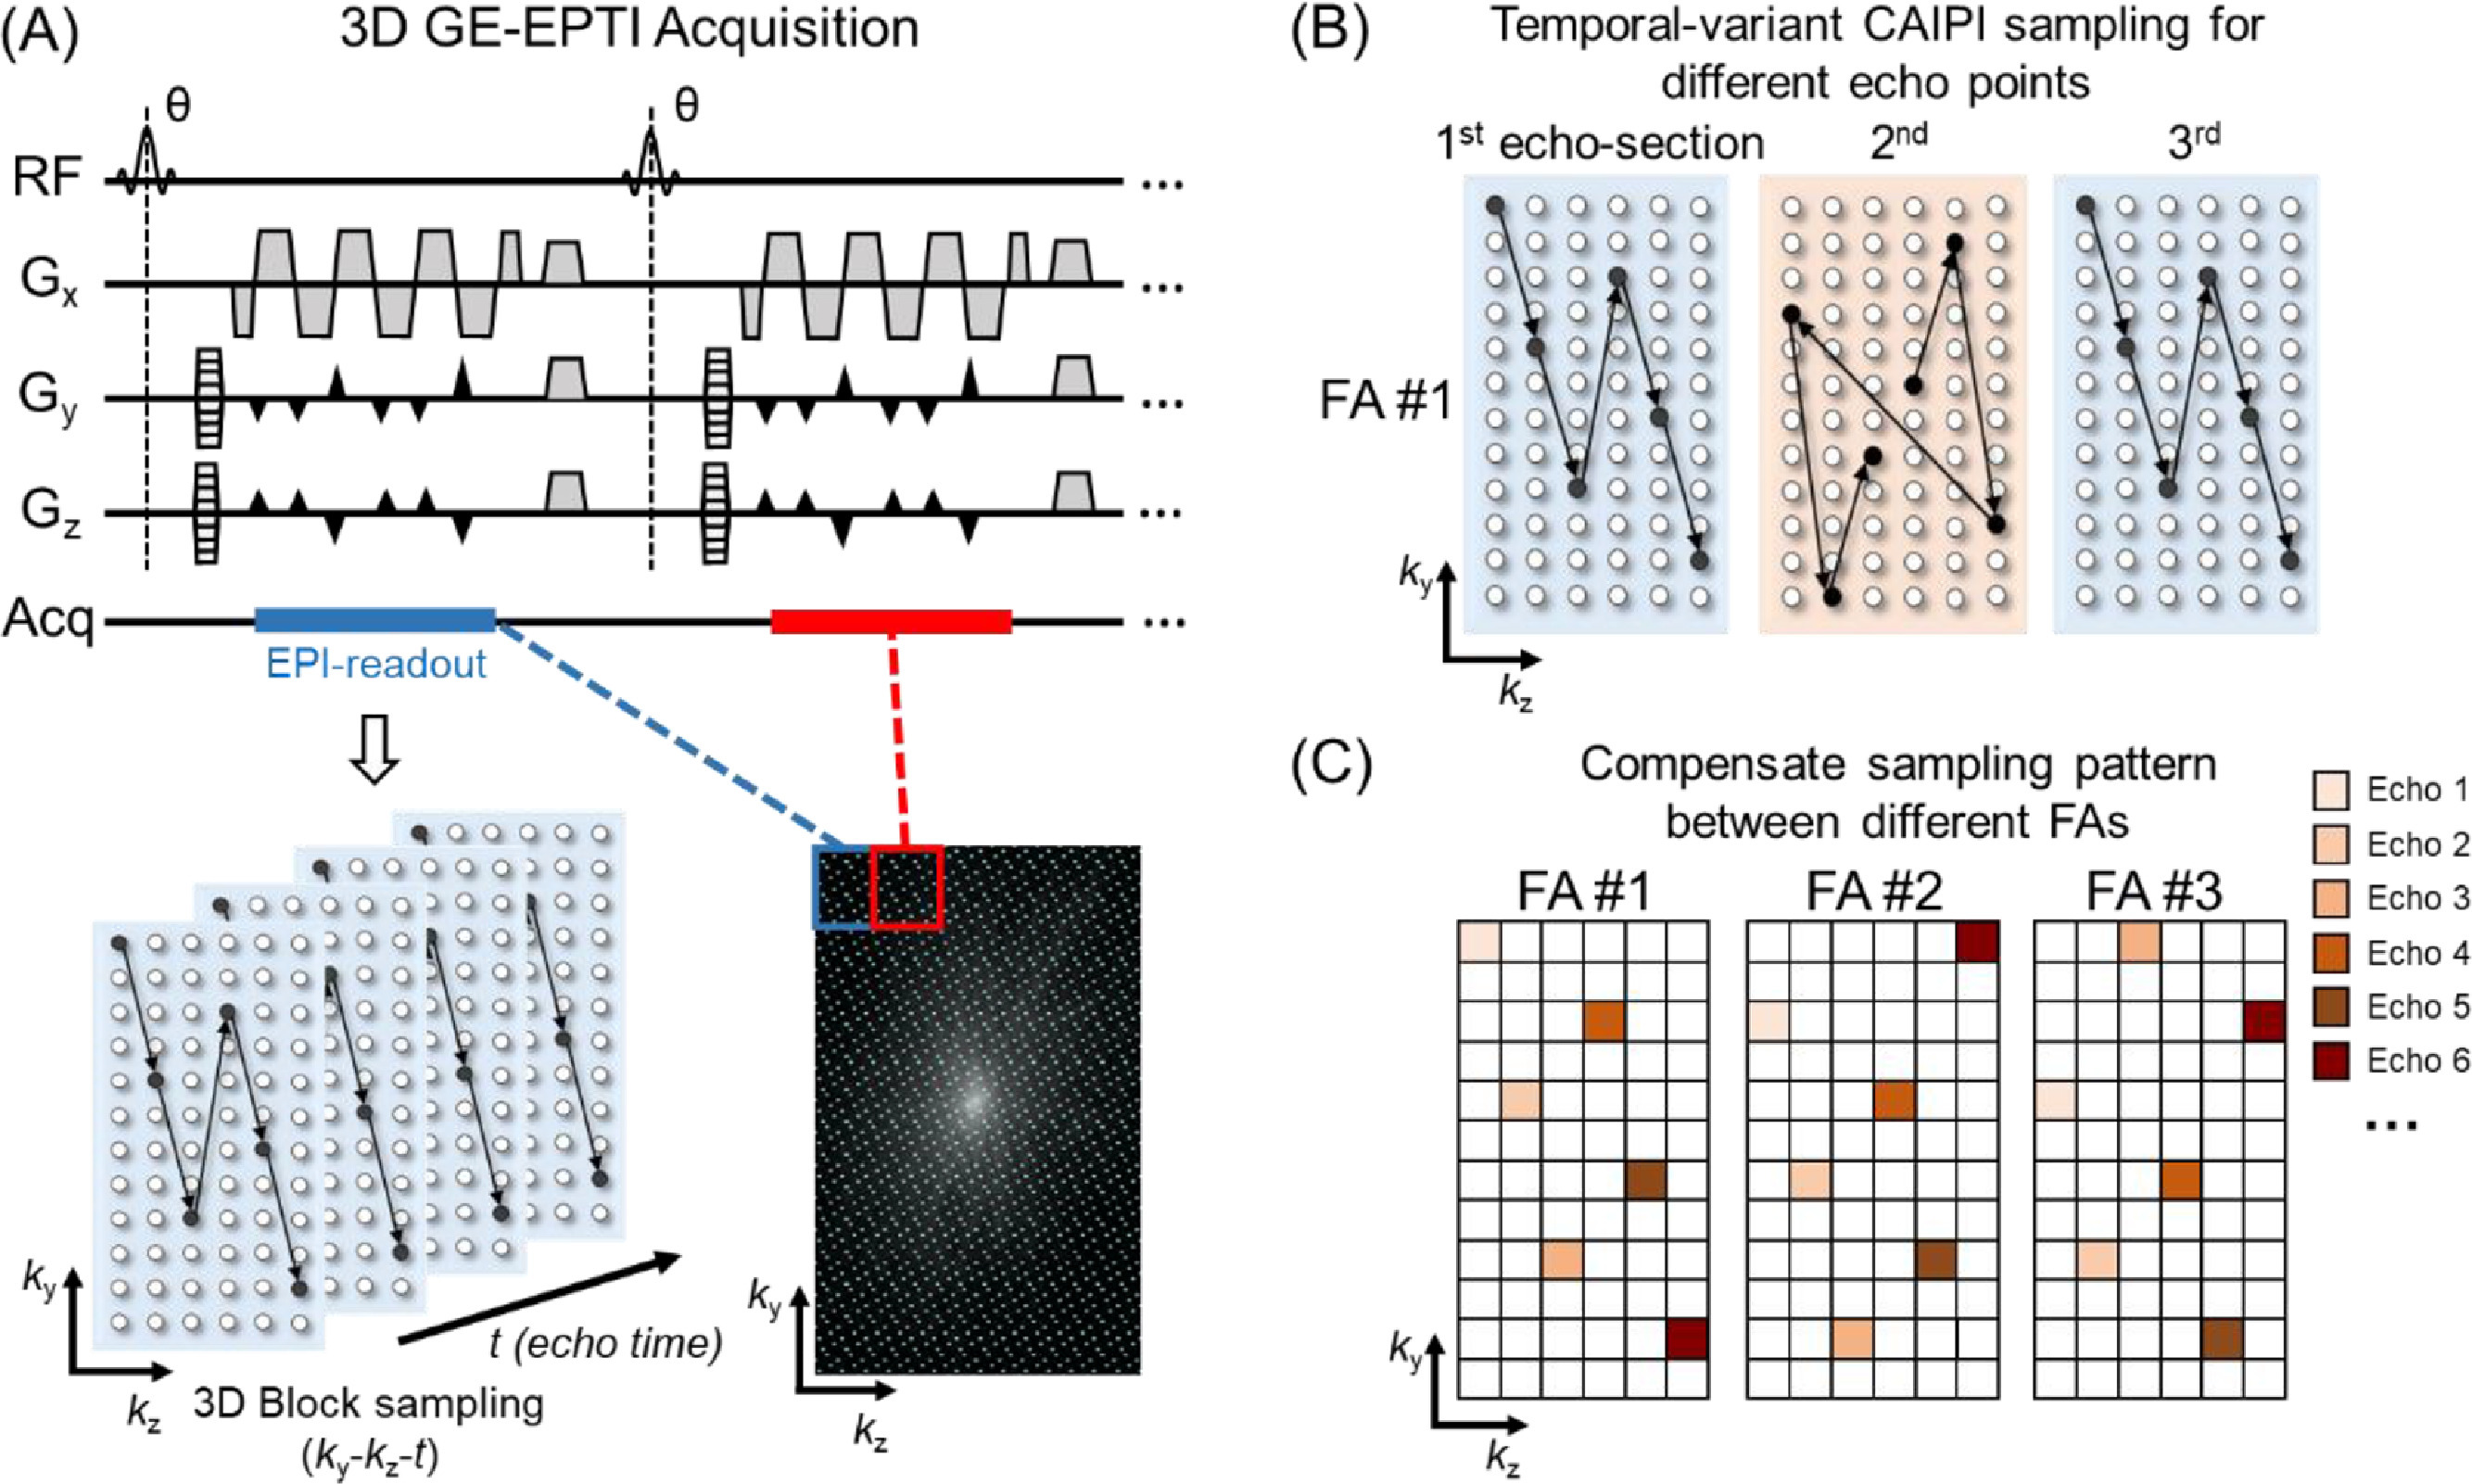
\includegraphics[width=0.64\textwidth]{vFA-EPTI_Sequence.jpg}
	\end{figure}
\end{frame}

\begin{frame}{EPTI Raw $k$-Space Data}
	ArrayShow \footnote{Sumpf T. \url{https://github.com/tsumpf/arrShow}.}:
	\begin{figure}
		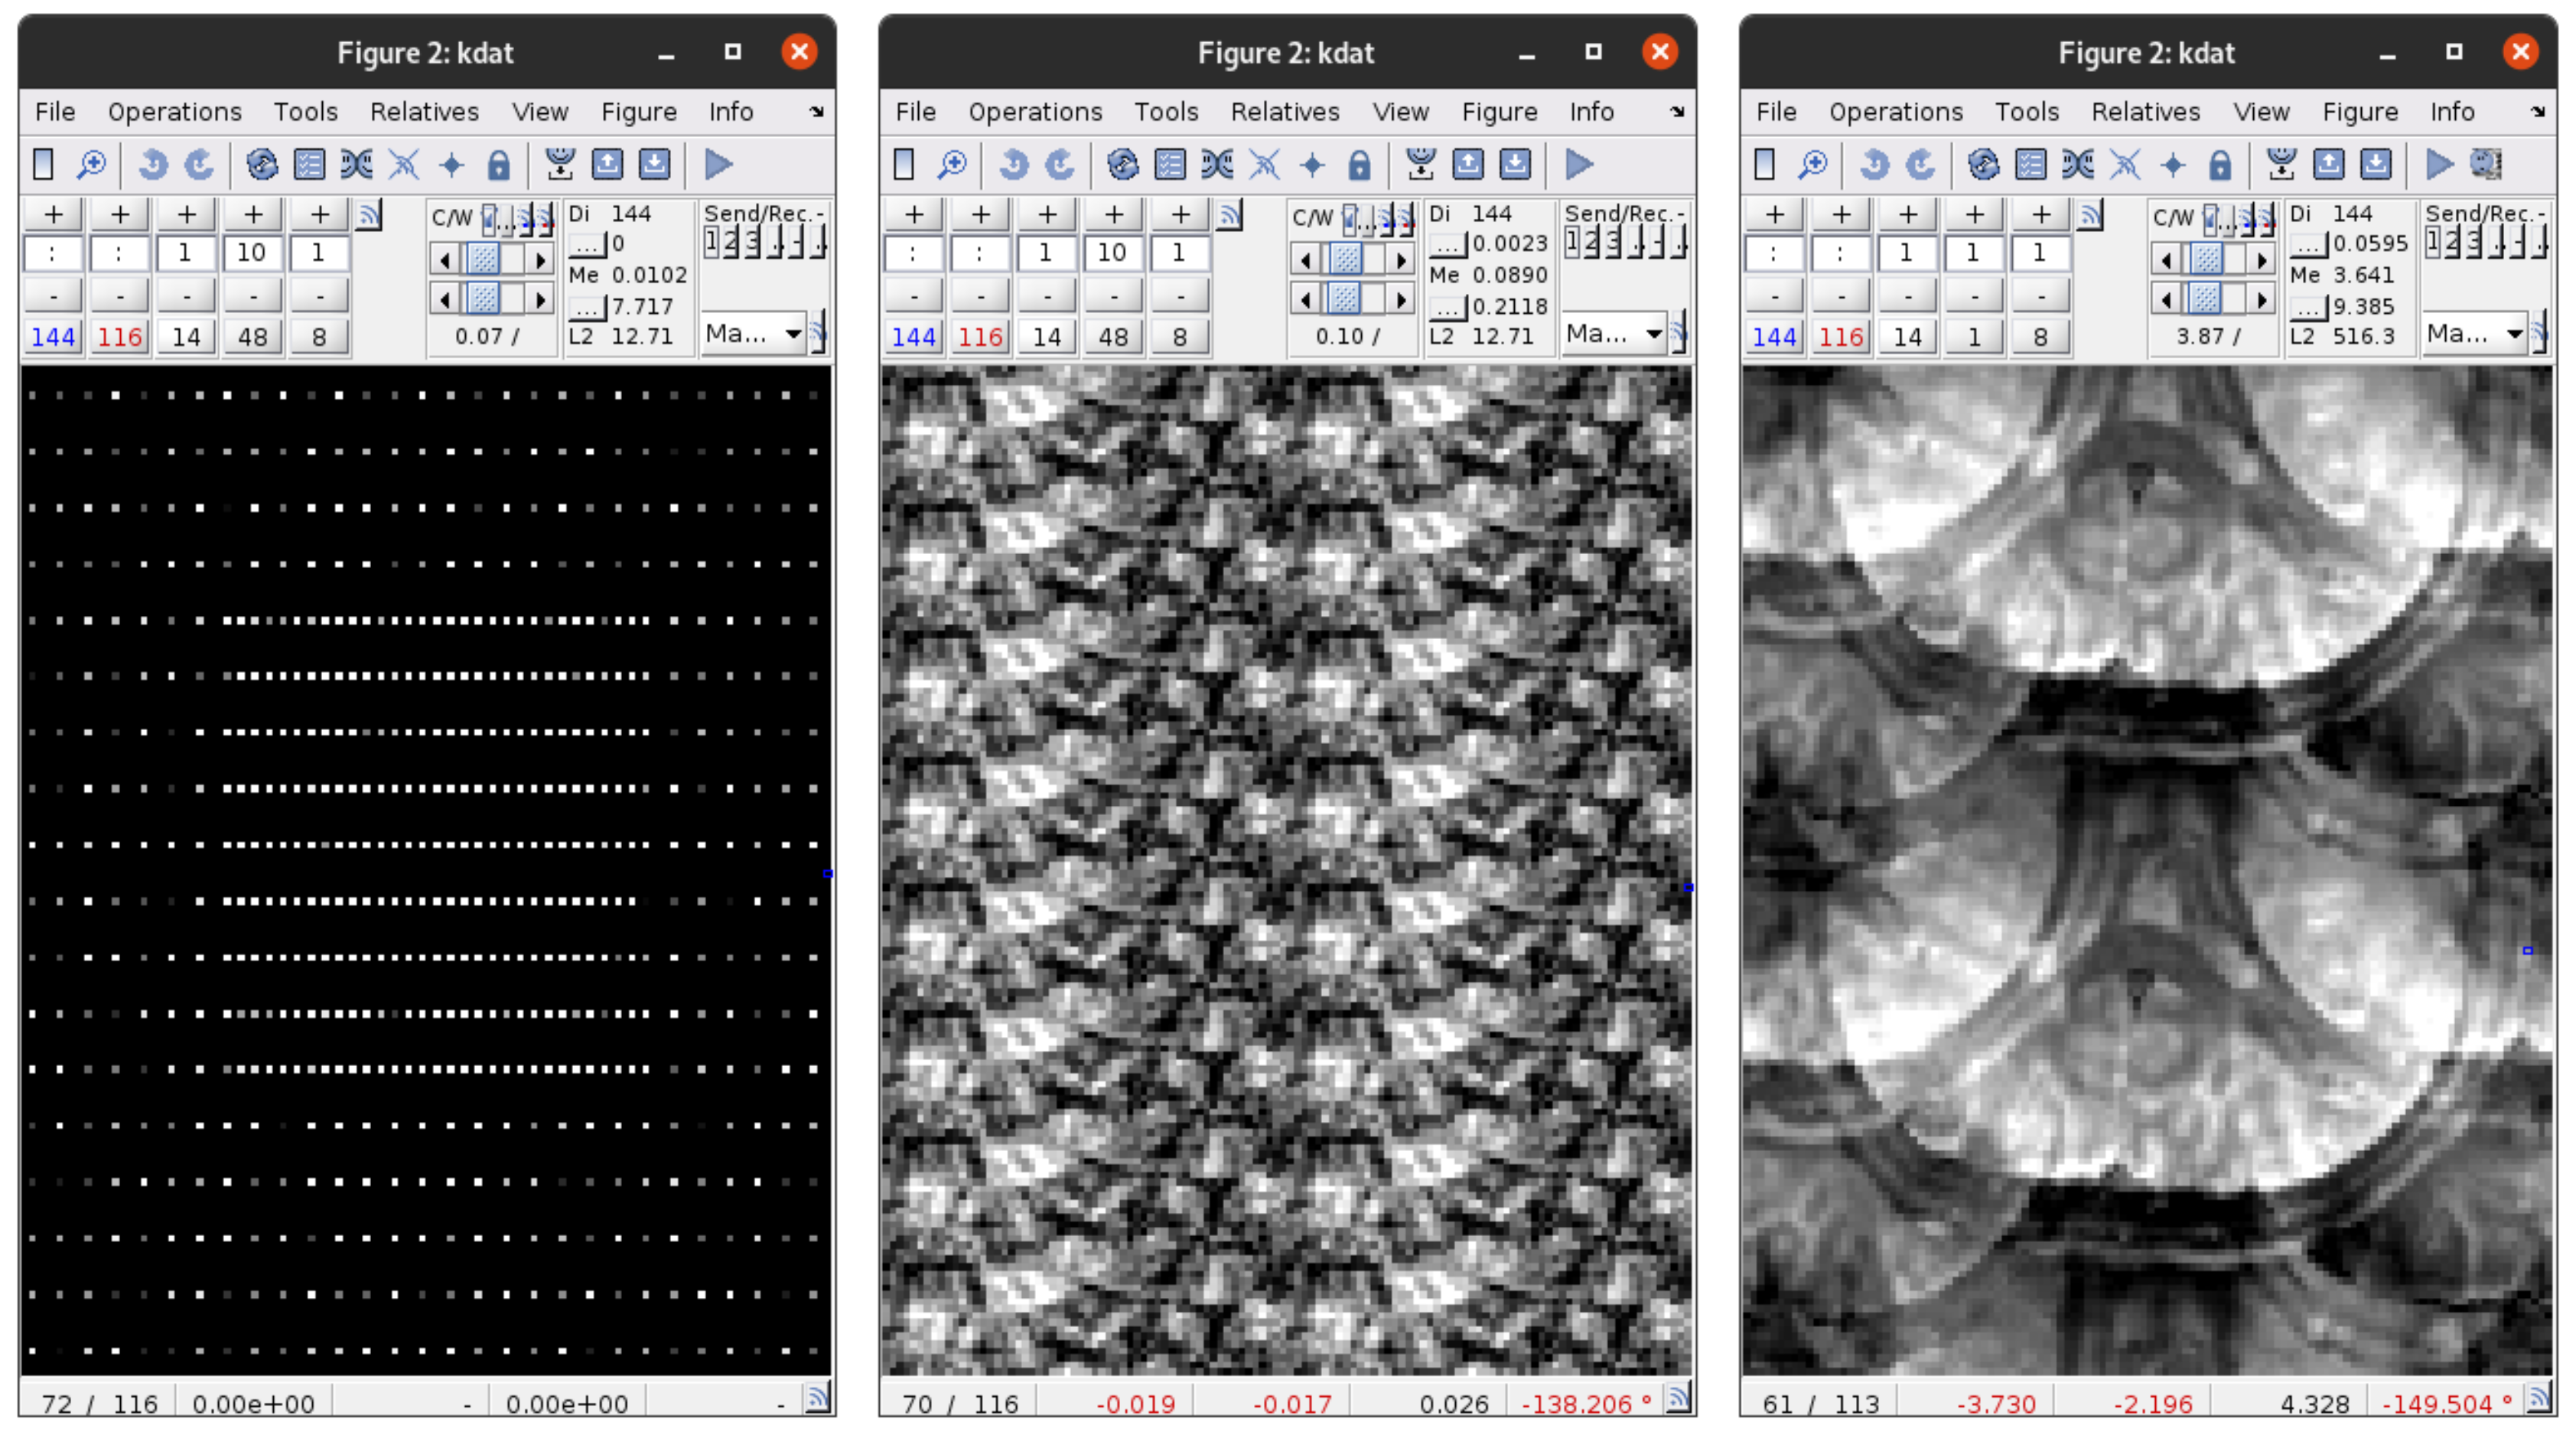
\includegraphics[width=0.7\textwidth]{vFA-EPTI_kdat_as.png}
	\end{figure}
\end{frame}

\begin{frame}[fragile]{Reproducing EPTI Subspace Reconstruction}
\begin{block}<1->{}
	{\large
	\begin{equation}
		\argmin_\alpha \norm{ y - \mathcal{F}_u S \Phi \hat{U} \alpha } + \lambda \norm{\text{LLR}(\alpha)}_1
	\end{equation}
	\begin{itemize}
		\item [$\diamond$] $\hat{U} \alpha$ presents multi-echo multi-flip-angle images.
		\item [$\diamond$] $\Phi = e^{i2\pi f_{B_0} \text{TE}_m}$~with $f_{B_0}$ being the 2D $B_0$ field inhomogeneity map, which is estimated from reference scans.
		\item [$\diamond$] Both $\hat{U}$ and $\Phi$ can be implemented 
		via the linop.Multiply(...) function in SigPy.
	\end{itemize}}
\end{block}

\begin{block}<2->{}
\begin{lstlisting}
img = app.SubspaceSenseRecon(kdat, coil, coil_dim=1,
                             lamda=0.005, regu='LLR',
                             basis=U, phase=phase,
                             blk_shape=(4, 8), blk_strides=(4, 8),
                             max_iter=20, solver='ADMM', rho=0.1,
                             device=backend.Device(0),
                             show_pbar=False).run()
\end{lstlisting}
\end{block}

\end{frame}

\begin{frame}{Reproducing EPTI Subspace Reconstruction}
The first six subspace coefficient maps:
\begin{figure}
	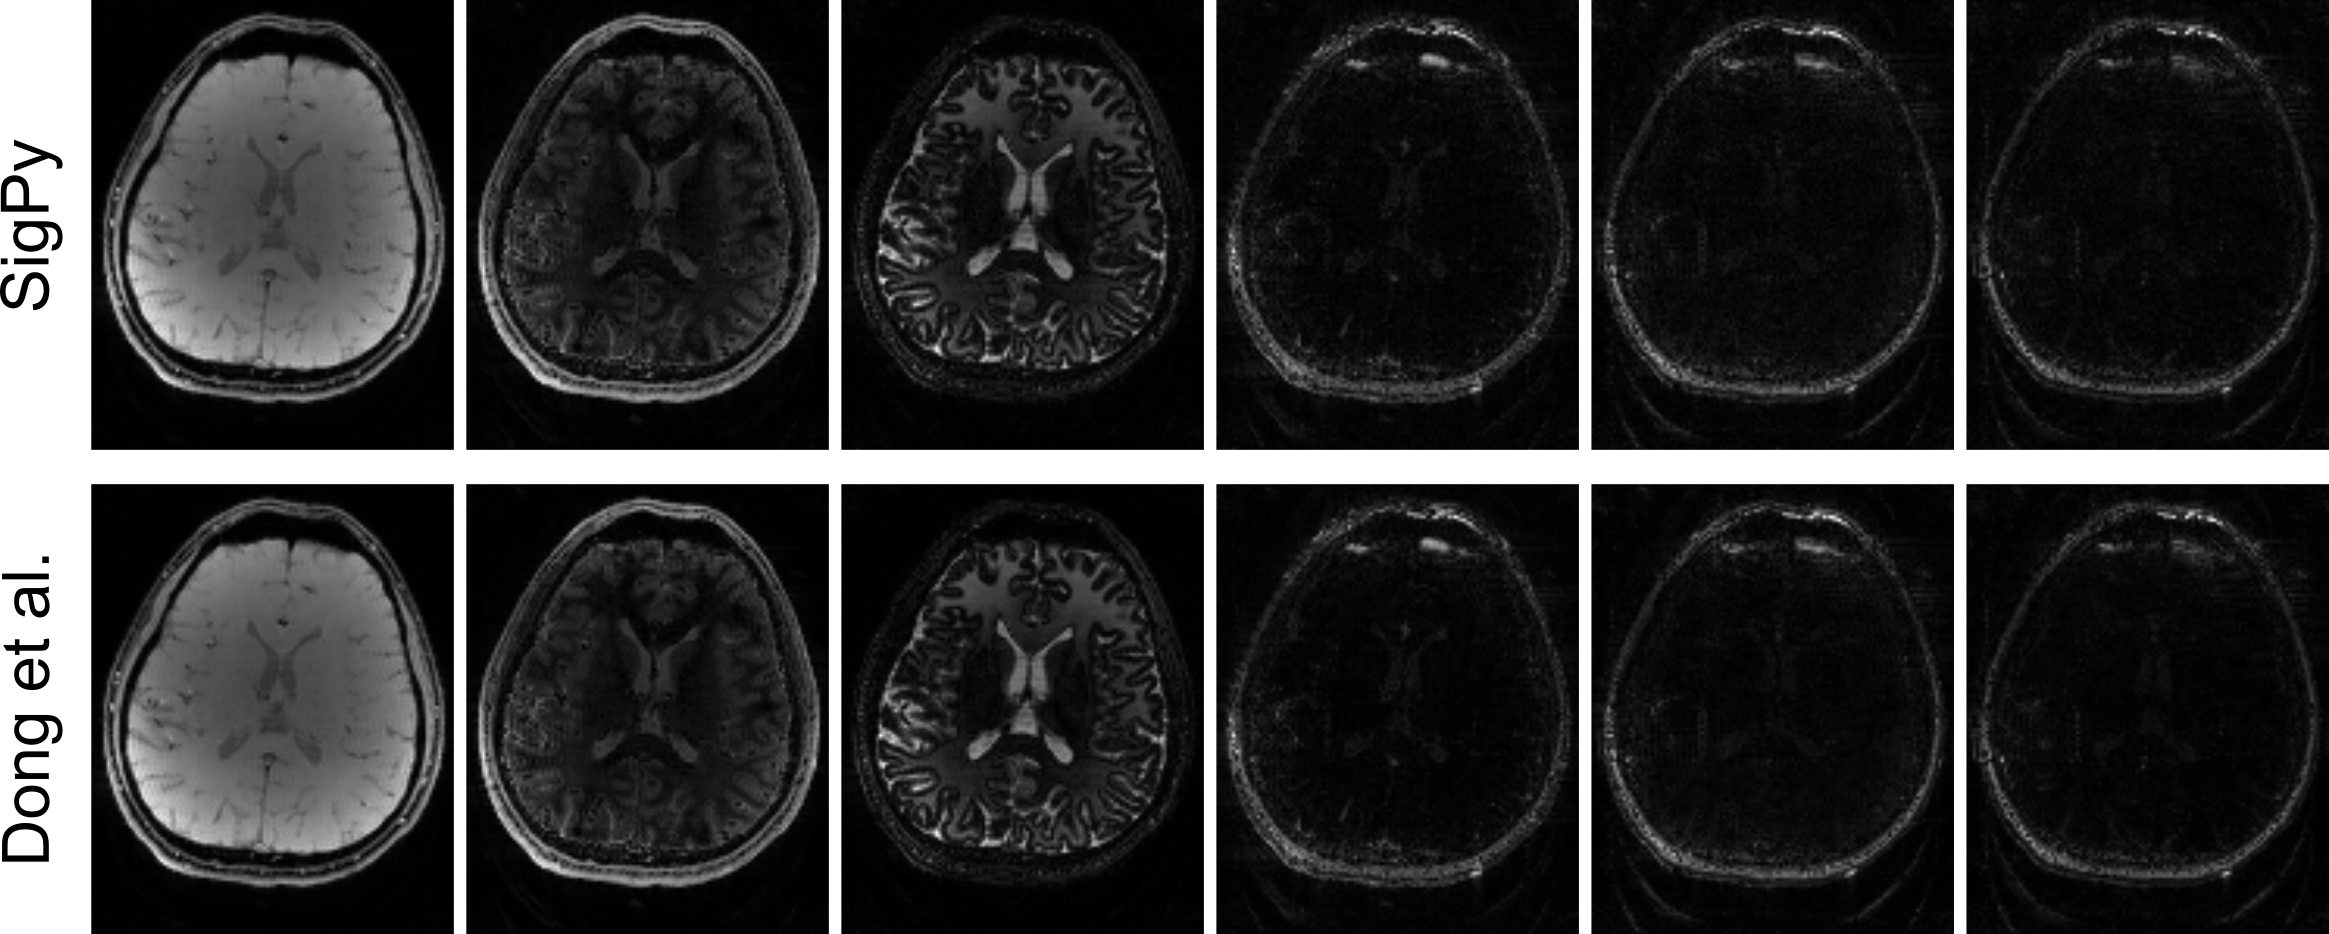
\includegraphics[width=\textwidth]{vFA-EPTI_comp.png}
\end{figure}
\end{frame}

\subsection{Radial Echo Planar Imaging (REPI)}
%=================================================================================

\begin{frame}{REPI \footnote{Tan Z, et al. Dynamic water/fat separation and $B_0$ inhomogeneity mapping - joint estimation using undersampled triple-echo multi-spoke radial FLASH. \textit{Magn Reson Med} (2019).} Sequence Design}
	\begin{figure}
		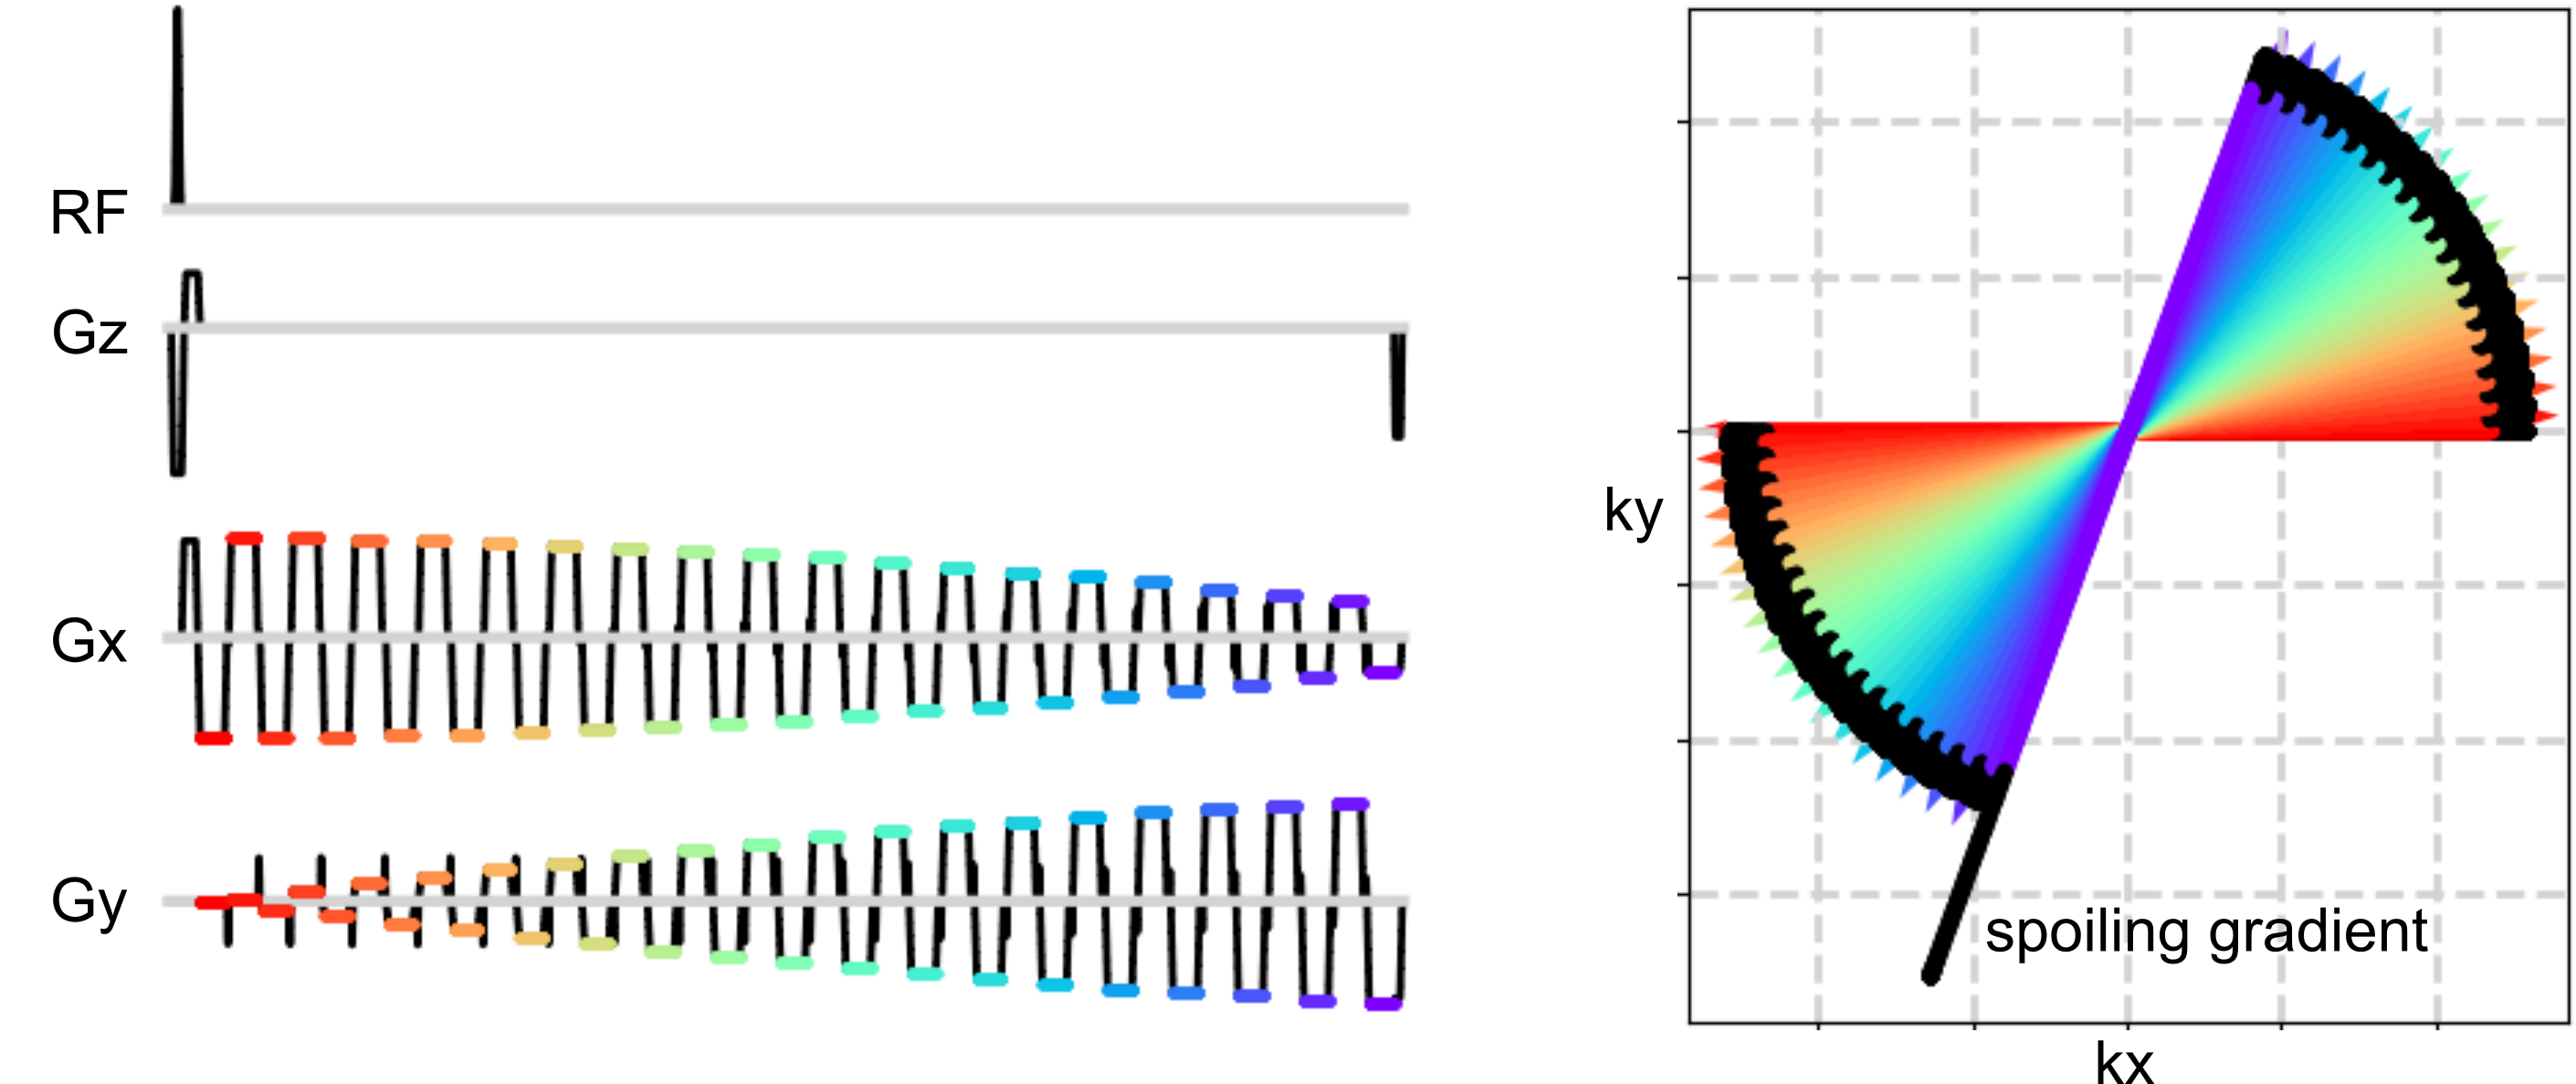
\includegraphics[width=0.9\textwidth]{REPI_Sequence.png}
	\end{figure}
\end{frame}

\begin{frame}{REPI Sequence Design}

\begin{block}{REPI Acquisition Parameters:}
{\large
	\begin{itemize}
		\item [$\diamond$] flip angle 4 degree
		\item [$\diamond$] 1~mm$^3$ isotropic resolution
		\item [$\diamond$] image matrix $220 \times 220 \times 192$
		\item [$\diamond$] 192 slices with stack-of-stars 3D sampling 
		\footnote{Block KT, et al. Towards routine clinical use of radial stack-of-stars 3D gradient-echo sequences for reducing motion sensitivity. \textit{J Korean Soc Magn Reson Med} (2014).}
		\item [$\diamond$] 7 shots per partition (slice)
		\item [$\diamond$] 35 echoes per shot with TE from 1.70 to 55.7~ms and TR 57.4~ms
		\item [$\diamond$] total scan time 1.3~minutes
		\item [$\diamond$] No reference scans.
		\vspace{1em}
		\item [$\rightarrow$] Acceleration factor: $R = 0.5\pi \times 220 /7 \approx 49$.
	\end{itemize}
}
\end{block}

\end{frame}

\begin{frame}{REPI with Density-Compensated Adjoint NUFFT Reconstruction}
{\large
\begin{columns}
\begin{column}{0.55\textwidth}
\begin{itemize}
	\item [$\diamond$] For non-Cartesian MRI, the $\mathcal{F}_u$ operator is implemented as linop.HDNUFFT, which creates a linop.NUFFT operator corresponding to every echo's sampling trajectory.
	\vspace{1em}
	\item [$\diamond$] Displayed images are echo- and coil-combined via root sum of square.
\end{itemize}
\end{column}

\begin{column}{0.45\textwidth}
\begin{figure}
	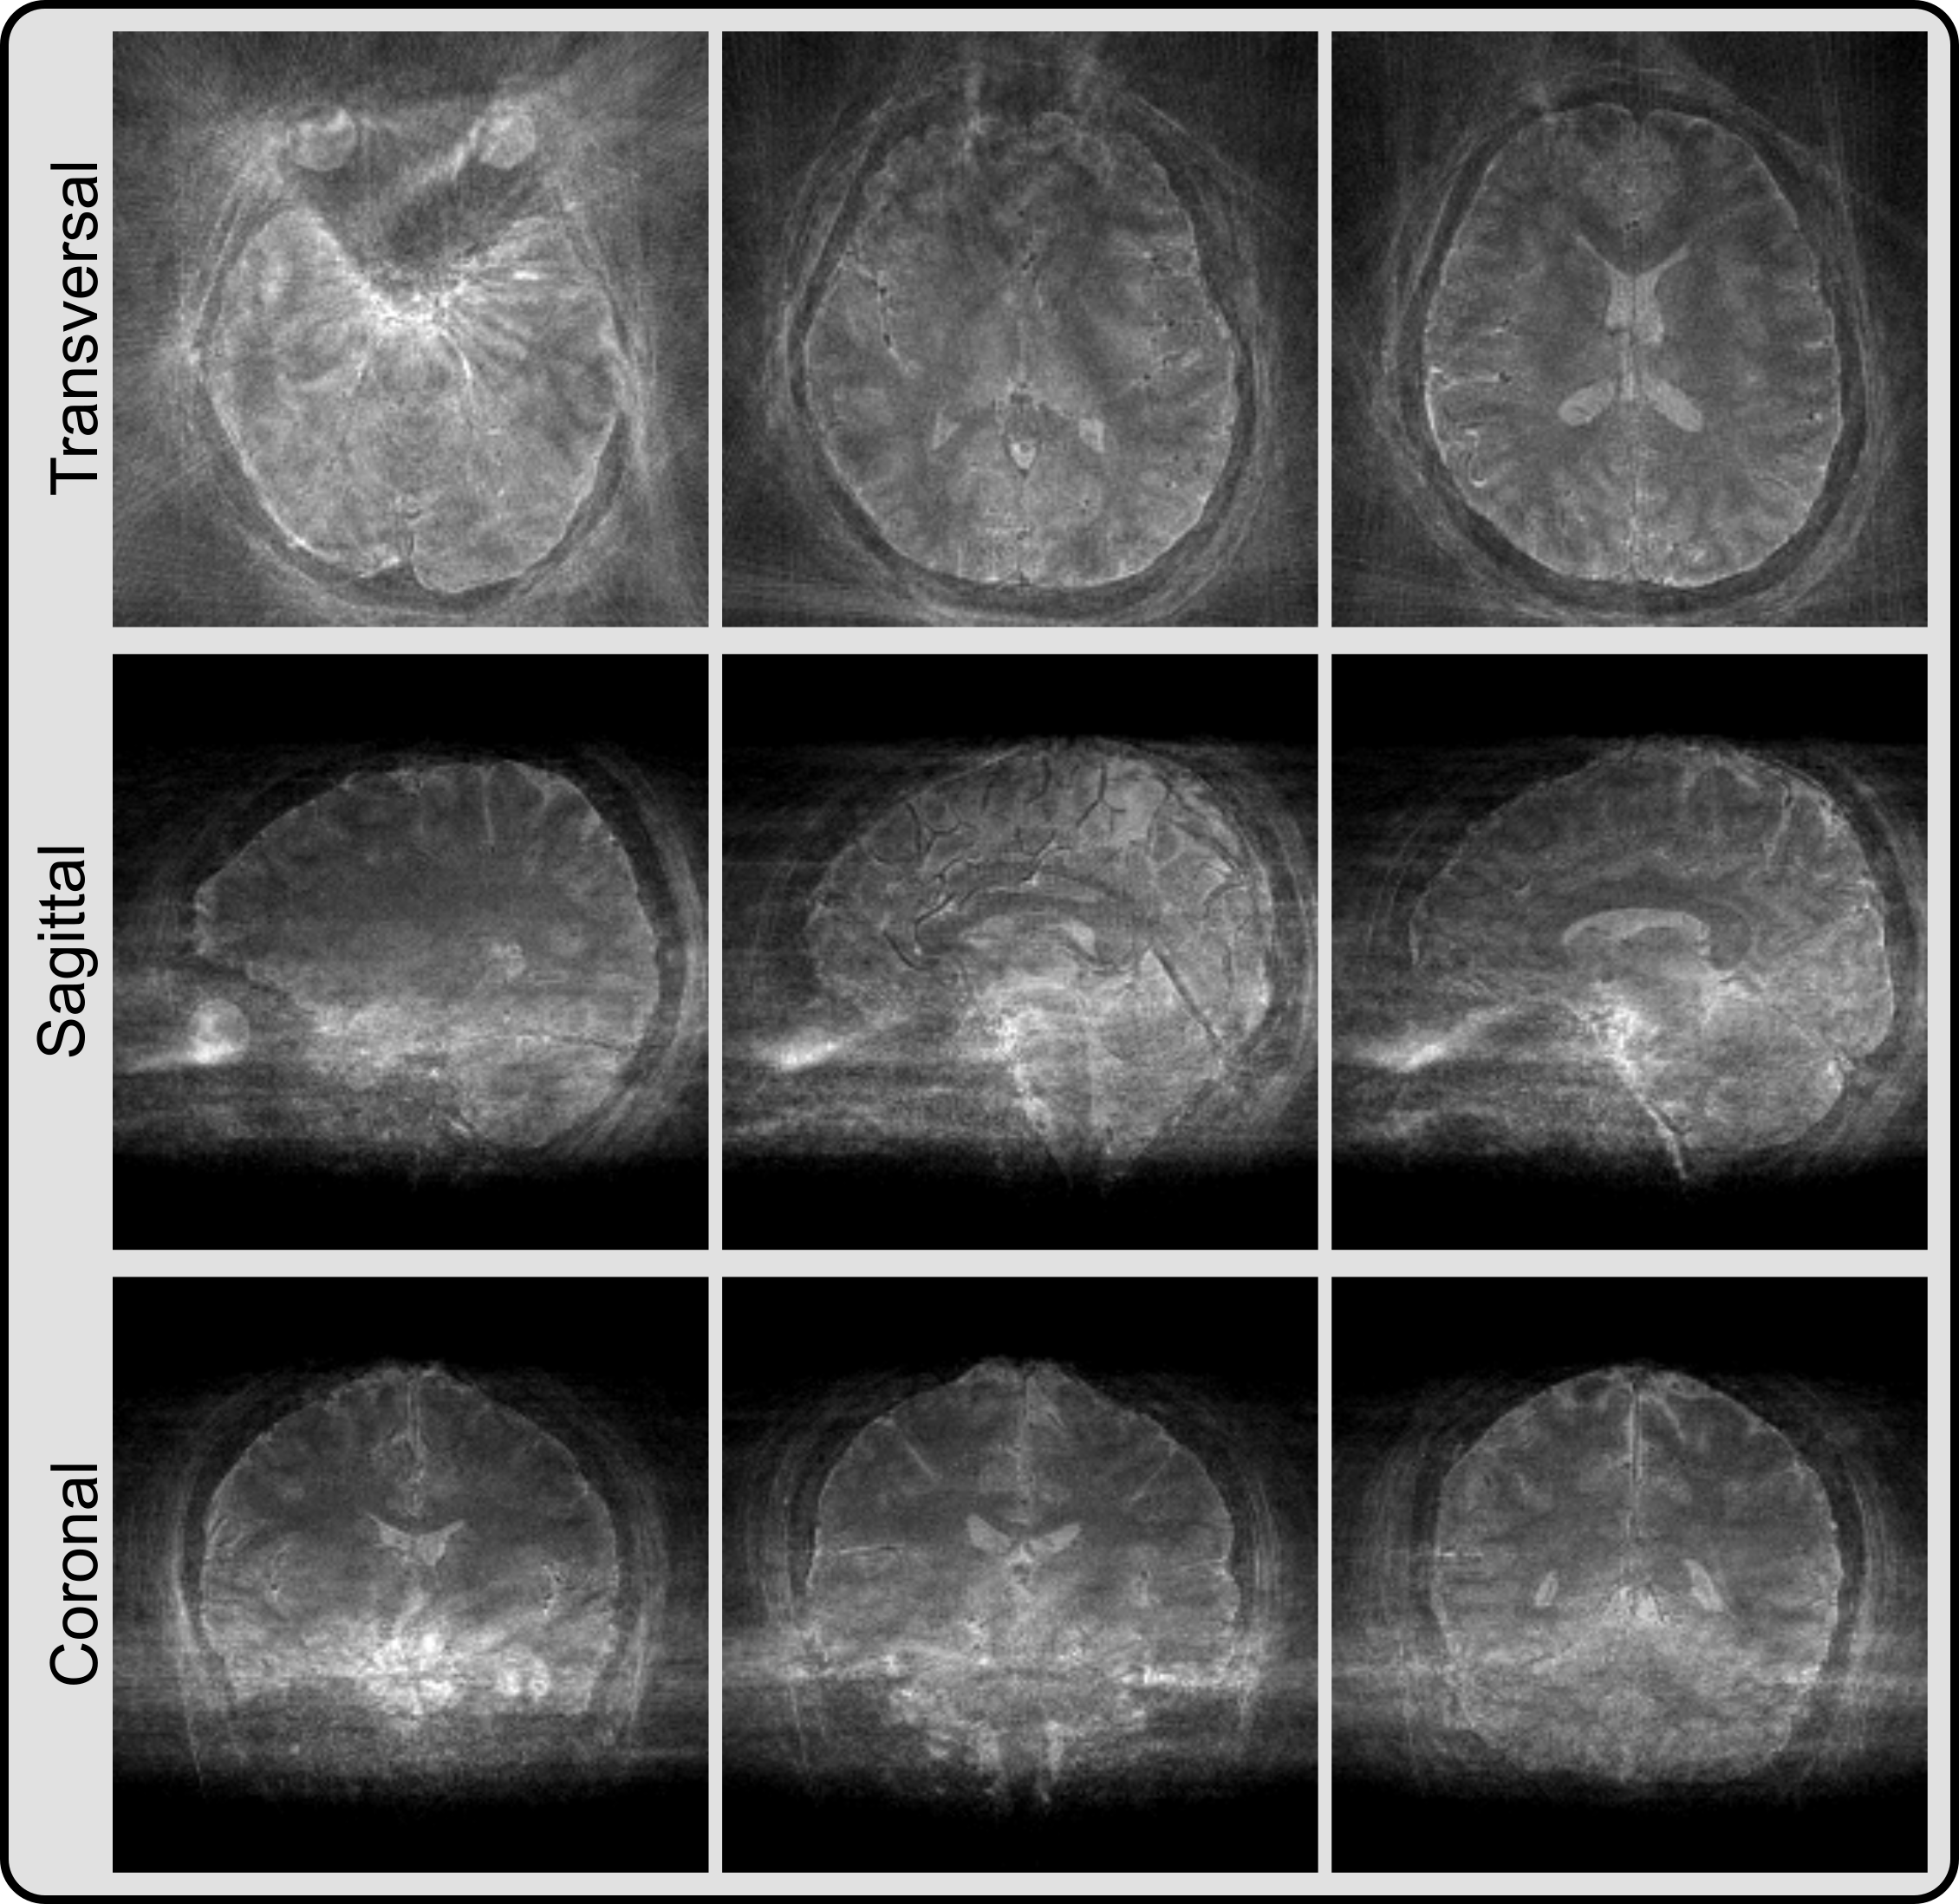
\includegraphics[width=\columnwidth]{REPI_nufft.png}
\end{figure}
\end{column}

\end{columns}}
\end{frame}


\begin{frame}[fragile]{REPI with Linear Subspace Modeling}
{\large
\begin{block}<1->{Build Dictionary}
\begin{equation}
	s_m = \rho \cdot e^{- \text{TE}_m / T_2^*} \cdot e^{i 2\pi f_{B_0} \text{TE}_m}
\end{equation}
\begin{itemize}
	\item [$\diamond$] $\rho$: set as scalar $1$.
	\item [$\diamond$] $T_2^*$: linearly distributed between 0.001 and 0.2~s with 100 atoms.
	\item [$\diamond$] $f_{B_0}$: linearly distributed between -50 and 50~Hz with 101 atoms.
\end{itemize}
\end{block}}

\begin{block}<2->{Extract Subspace Matrix $\hat{U}$}
\begin{lstlisting}
sig2 = np.reshape(sig, (sig.shape[-7], -1))
U, S, VH = np.linalg.svd(sig2, full_matrices=False)
U_sub = U[:, :num_coeffs]
recov_sig = U_sub @ U_sub.T @ sig2

err = get_rel_error(recov_sig, sig2)
\end{lstlisting}
\end{block}

\end{frame}


\begin{frame}{Larger $B_0$ Range Requires More Subspace Coefficients}
\begin{figure}
	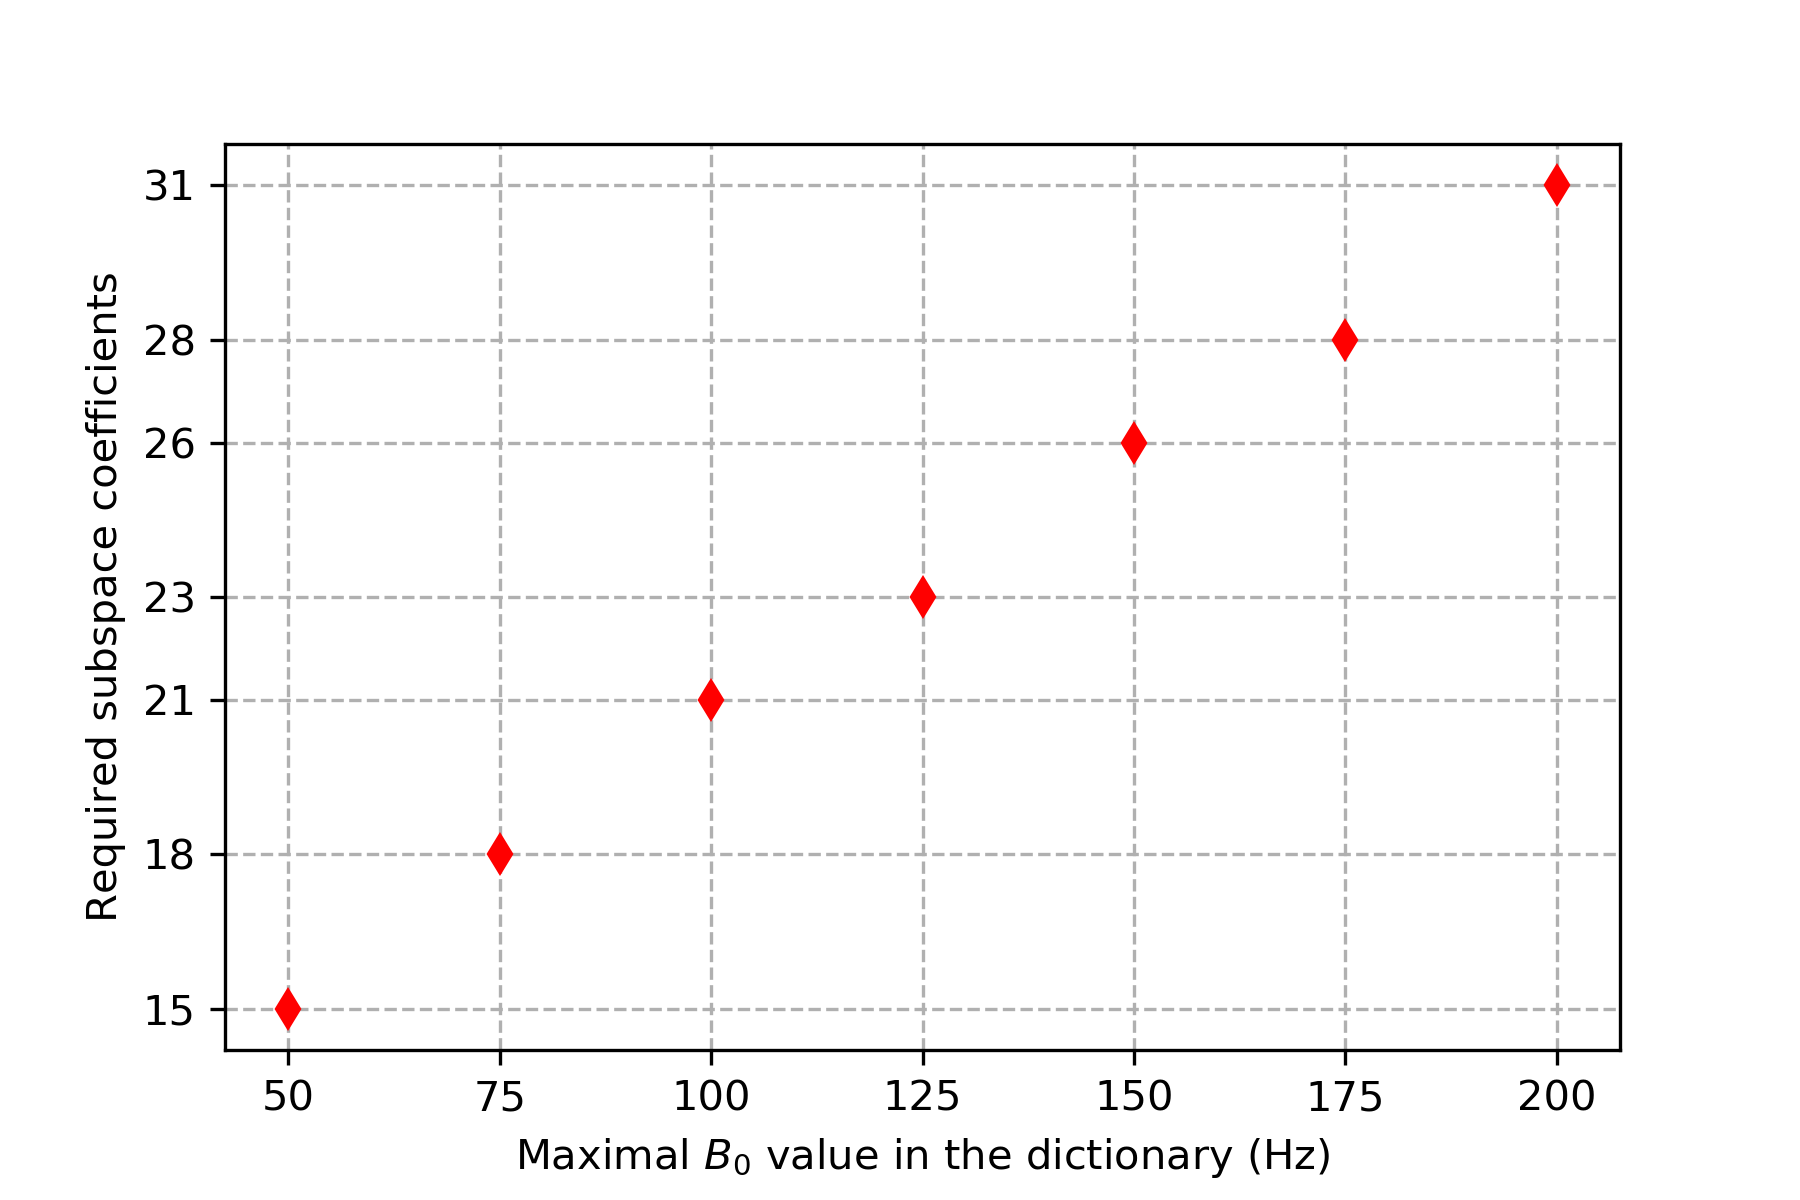
\includegraphics[width=0.7\textwidth]{REPI_subspace_model_1.png}
\end{figure}
\end{frame}


\begin{frame}{Effects of Insufficient Subspace Coefficients}
\begin{figure}
	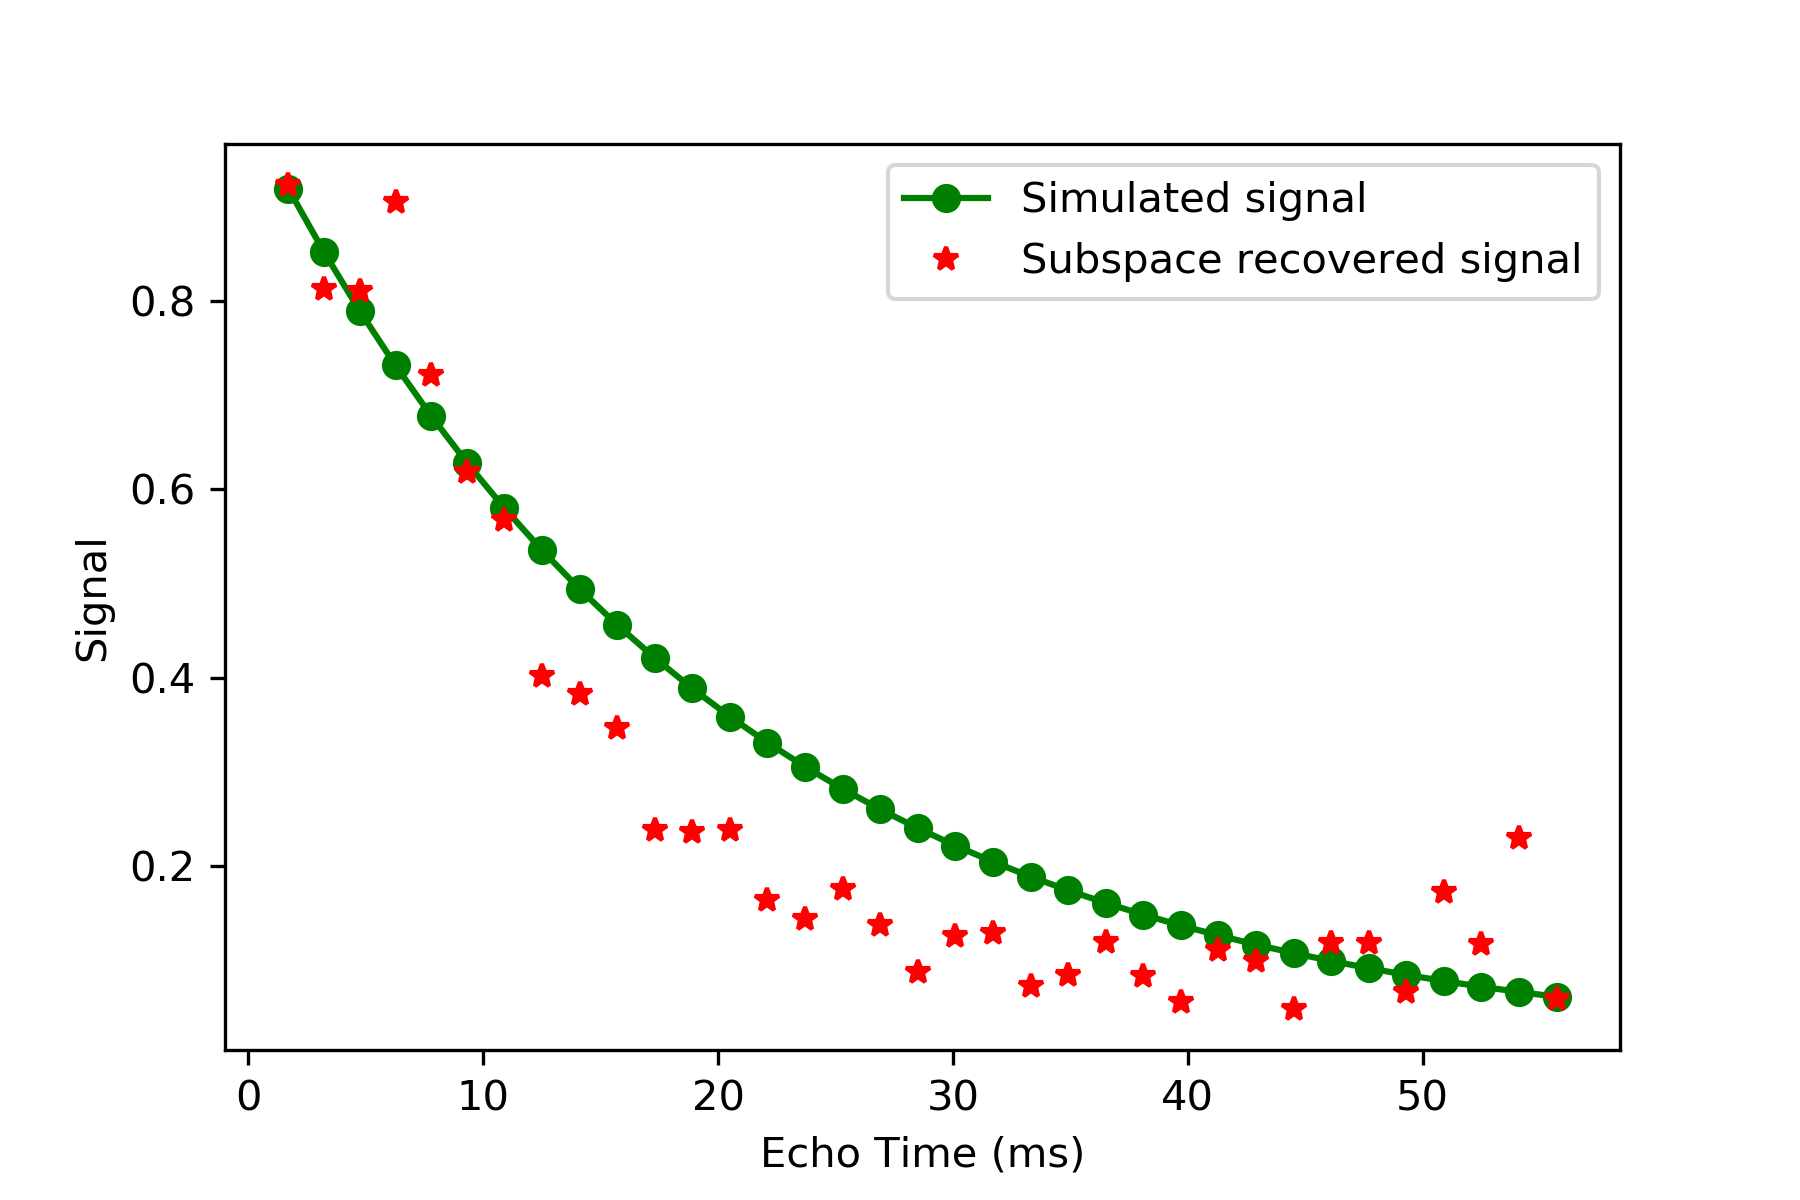
\includegraphics[width=0.7\textwidth]{REPI_subspace_model_2.png}
\end{figure}
\end{frame}


\begin{frame}{REPI with LLR Regularized Linear Subspace Reconstruction}
\begin{columns}
\begin{column}{0.45\textwidth}
\begin{figure}
	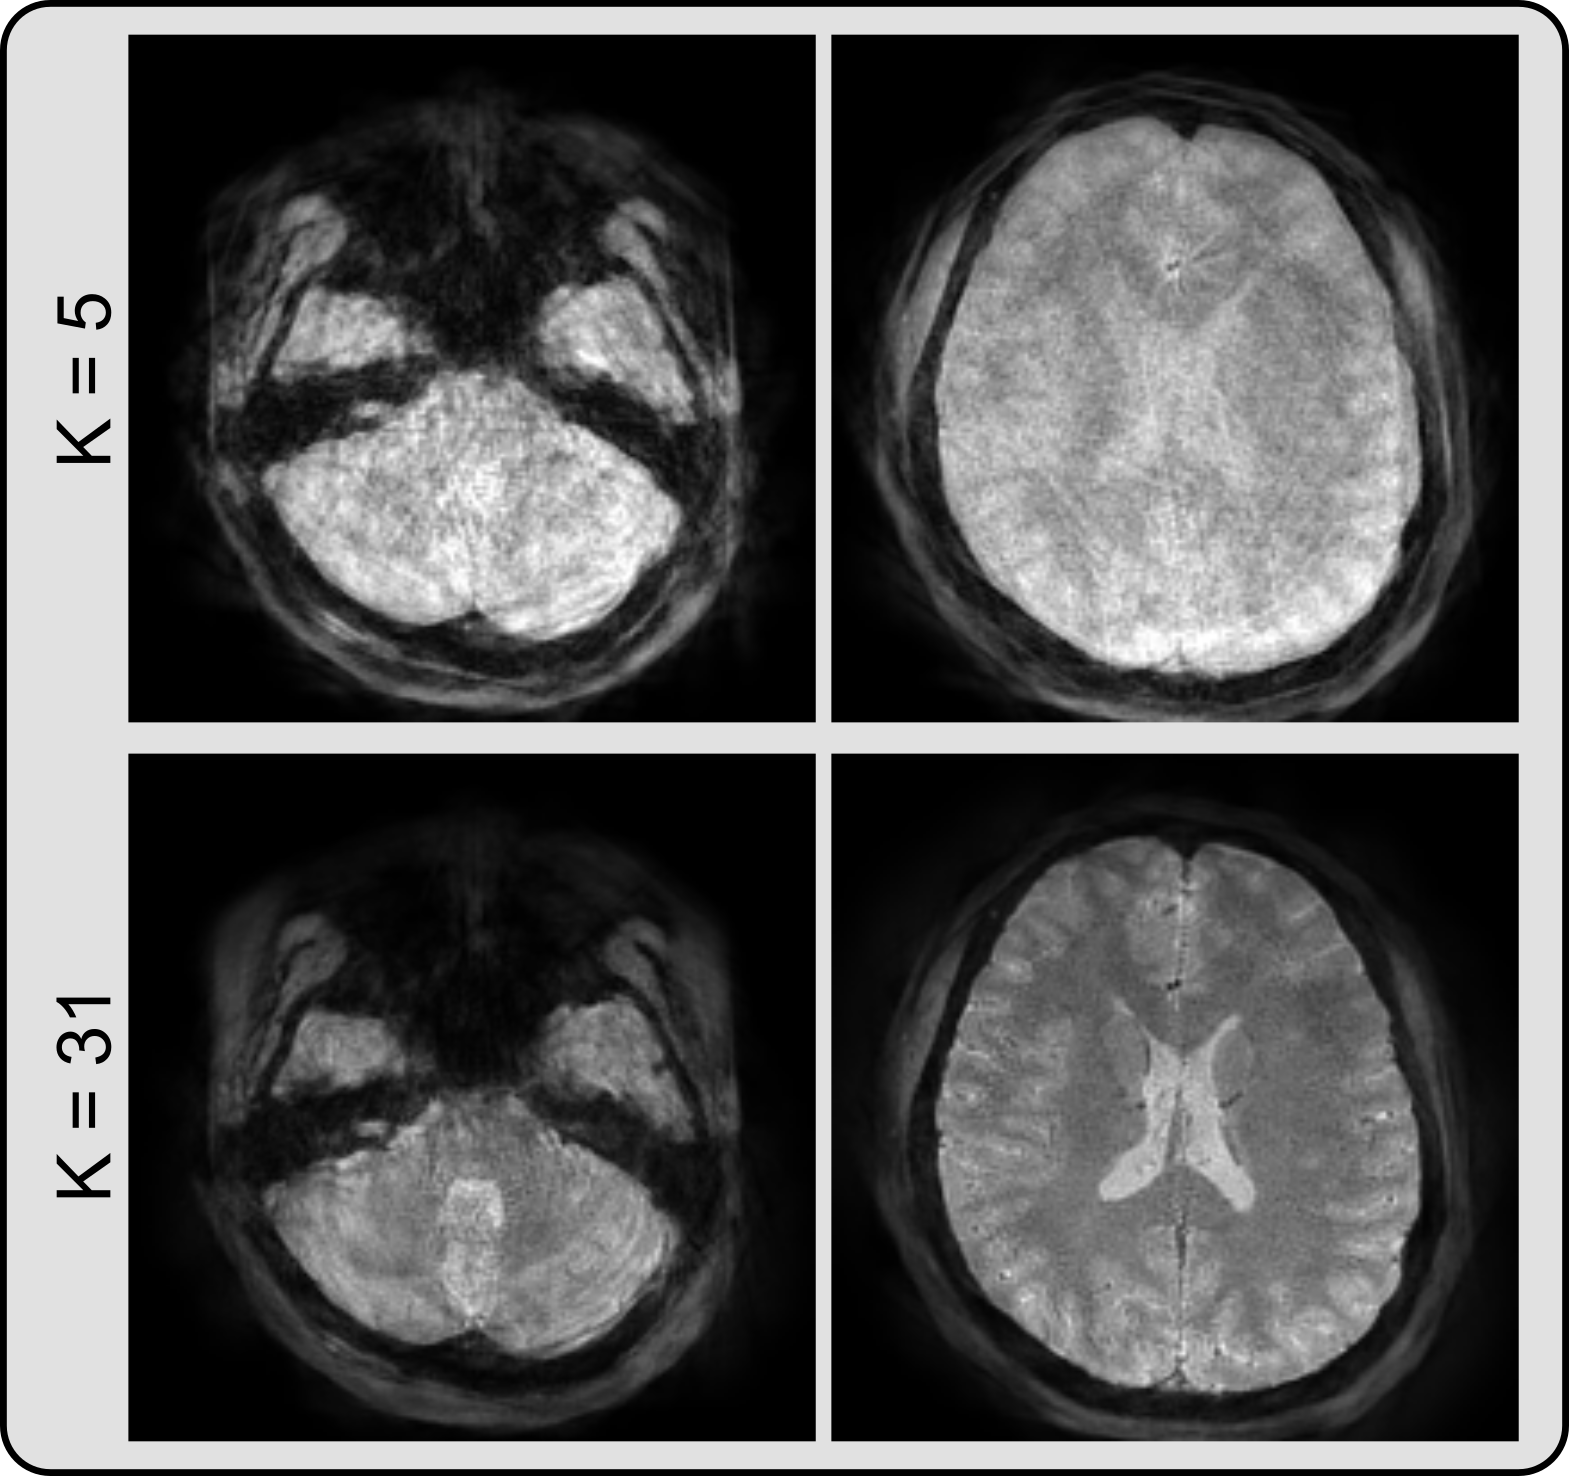
\includegraphics[width=\columnwidth]{REPI_coeffs.png}
\end{figure}
\end{column}

\begin{column}{0.55\textwidth}
{\large
\begin{itemize}
	\item [$\diamond$] Displayed are echo-combined images after reconstruction.
	\vspace{2em}
	\item [$\diamond$] Larger $K$ (number of subspace coefficients) is necessary 
	in the case of wide-range phase modulation in the dictionary of MGRE signal. 
	\vspace{2em}
	\item [$\diamond$] The reconstruction time per slice for $K = 5$ and $K = 31$ 
	was about 24 and 140 seconds, respectively.
\end{itemize}}

\end{column}
\end{columns}

\end{frame}


\begin{frame}{REPI with LLR Regularized Linear Subspace Reconstruction
	\footnote{Tan Z, et al. ISMRM 2022;1860.}}

\end{frame}


\begin{frame}{REPI with LLR Regularized Linear Subspace Reconstruction}
\begin{columns}
\begin{column}{0.6\textwidth}
\begin{figure}
	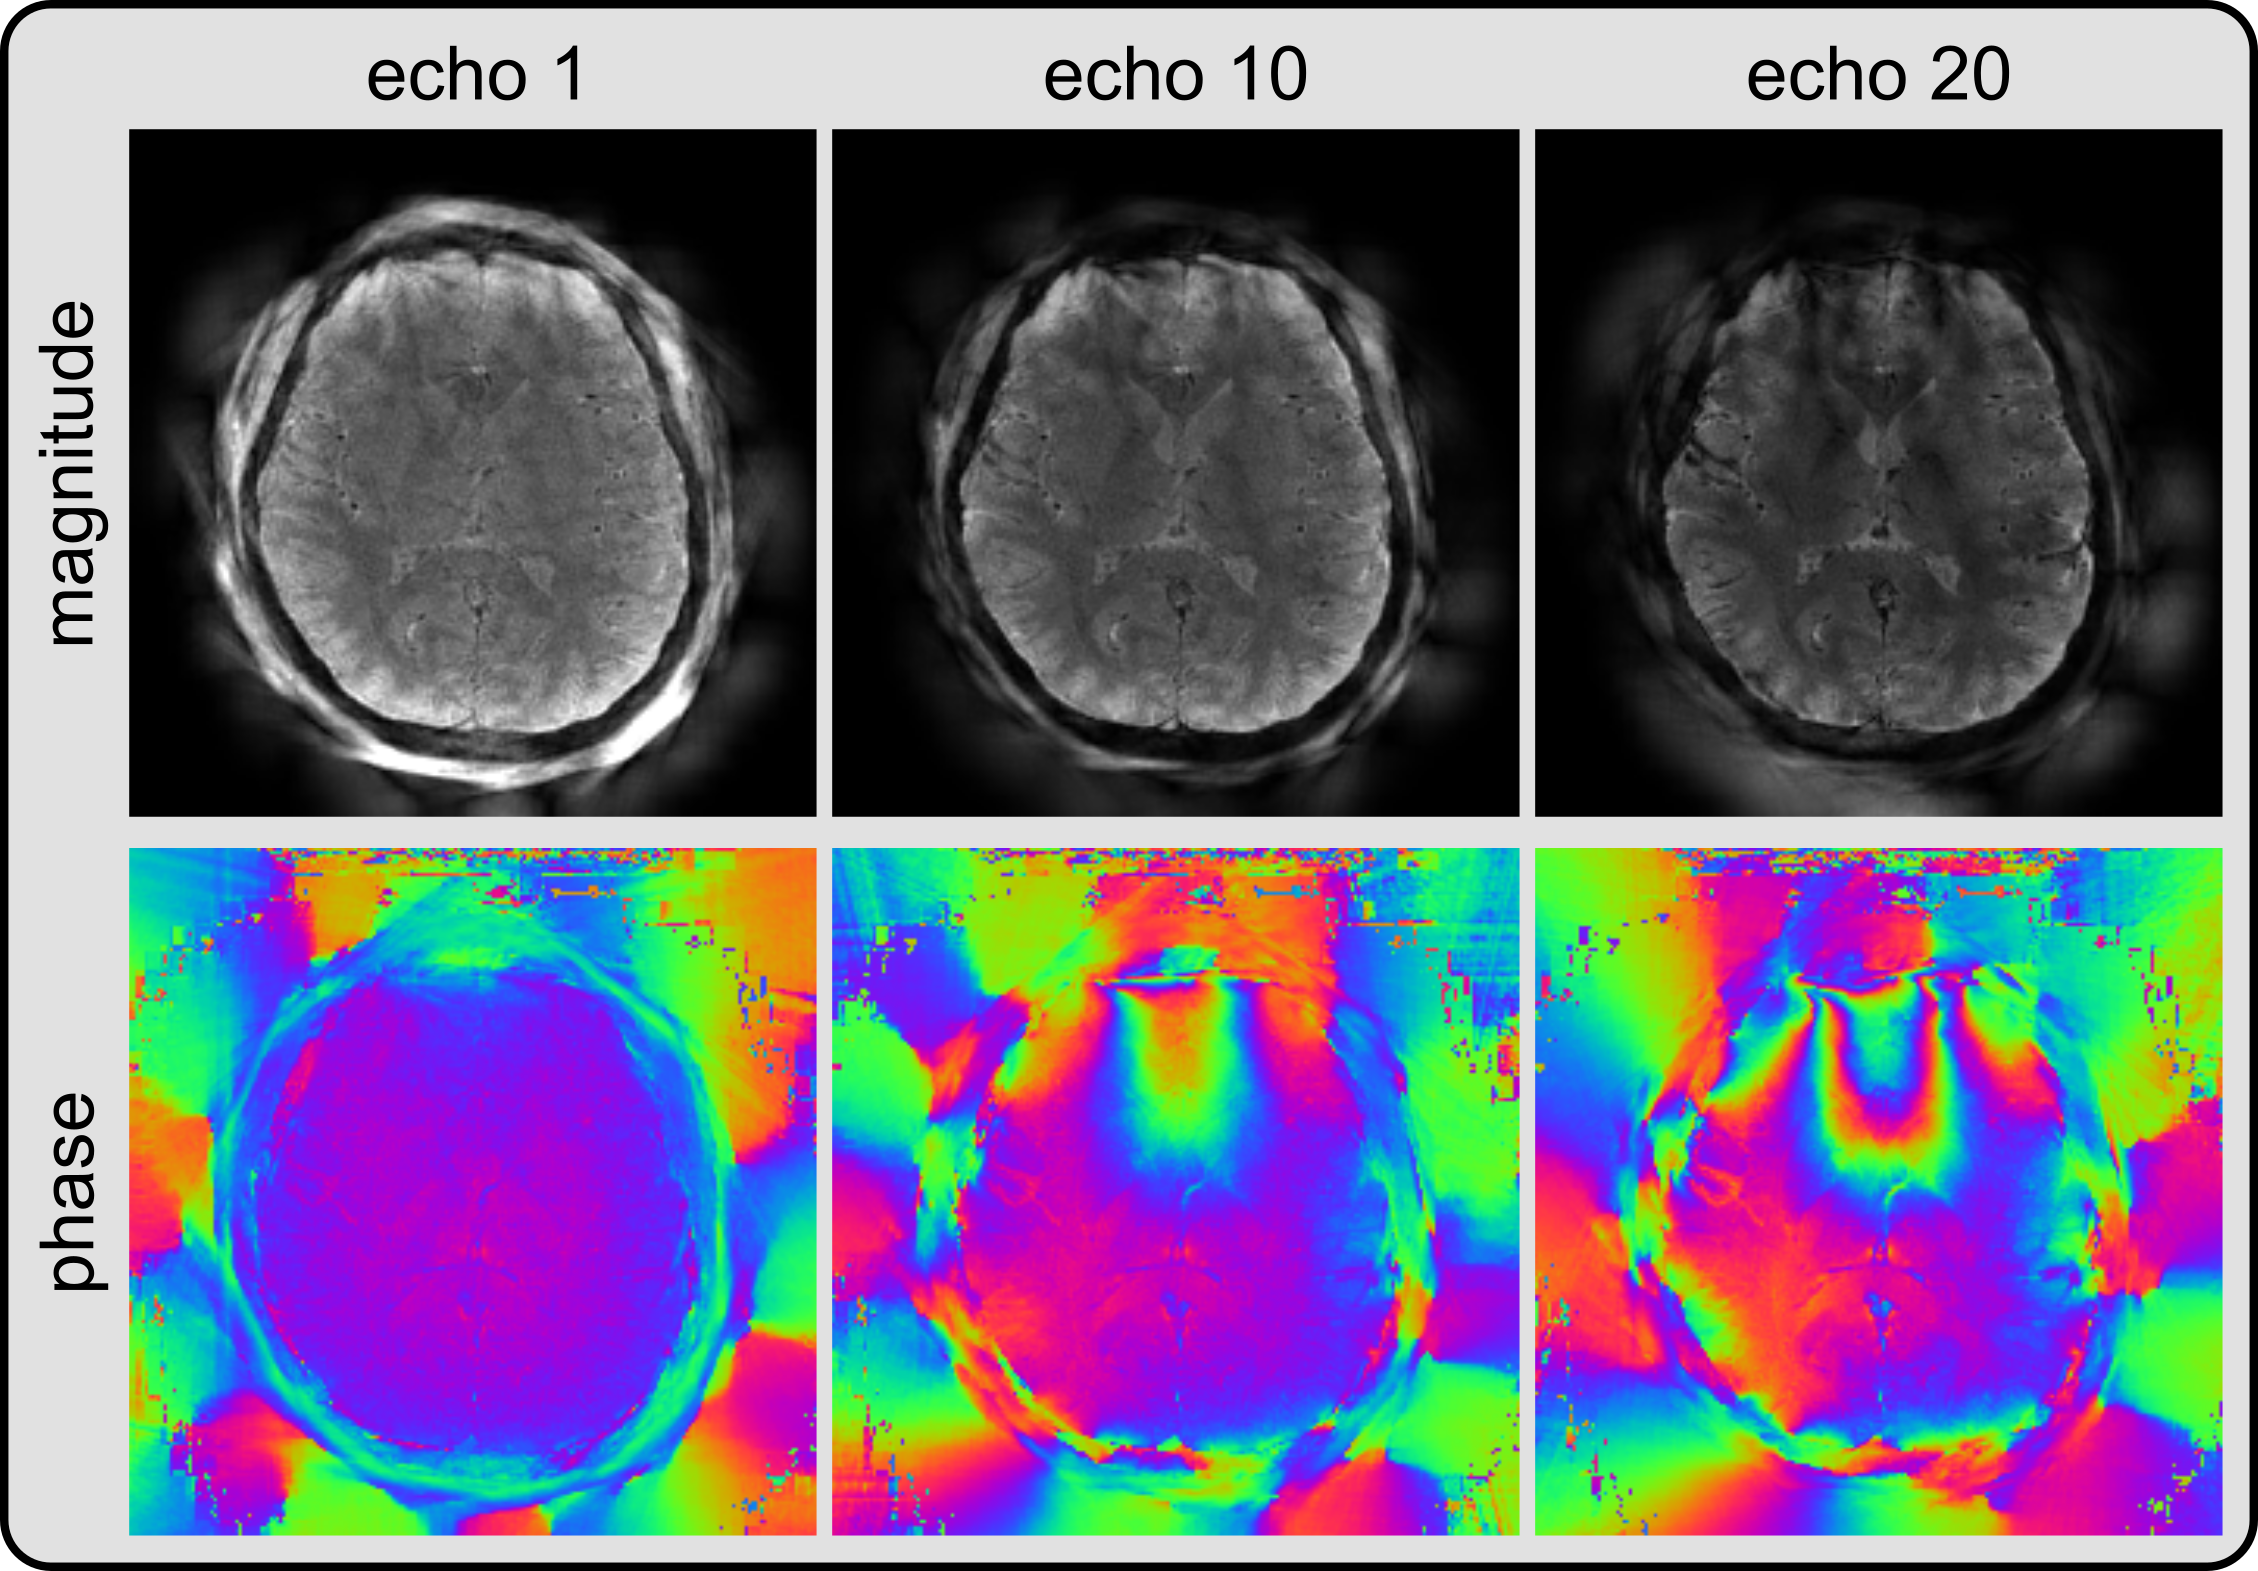
\includegraphics[width=\columnwidth]{REPI_echoes.png}
\end{figure}
\end{column}

\begin{column}{0.4\textwidth}
{\large
\begin{itemize}
	\item [$\diamond$] The magnitude and phase images 
	of the 1st, 10th, and 20th echoes.
	\vspace{2em}
	\item [$\diamond$] Linear phase evolution along echoes.
	\vspace{2em}
	\item [$\diamond$] Residual streaking artifacts.
\end{itemize}}
\end{column}
\end{columns}
\end{frame}